\documentclass[12pt]{article}

\usepackage{graphicx}
\usepackage{graphics}
\usepackage{multicol}
\usepackage{epsfig,amsmath,amsfonts}
\usepackage{xspace}
\usepackage{subfigure}

\makeatletter                                   % Make '@' accessible. 
\oddsidemargin=0in                              % Left margin minus 1 inch.
\evensidemargin=0in                             % Same for even-numbered pages.
\marginparsep=0pt                               % Space between margin & text

\renewcommand{\baselinestretch}{1.2}              % Double spacing

\textwidth=6.5in                                % Text width (8.5in - margins).
\textheight=9in                                 % Body height (incl. footnotes)

\topmargin=0in                                  % Top margin minus 1 inch.
\headsep=0.0in                                  % Distance from header to body.
\skip\footins=4ex                               % Space above first footnote.
\hbadness=10000                                 % No "underfull hbox" messages.
\makeatother                                    % Make '@' special again.

\newcommand{\mate}{Mat\'{e}\xspace}
\newcommand{\bomb}{Bombilla\xspace}

\title{Mat\'{e} Manual}
\author{Philip Levis\\pal@cs.berkeley.edu}
\date{}

\begin{document}

%\fontfamily{cmss}                               % Make text sans serif.
%\fontseries{m}                                  % Medium spacing.
%\fontshape{n}                                   % Normal: not bold, etc.
%\fontsize{10}{10}                               % 10pt font, 10pt line spacing 

\maketitle
\vspace{2in}
\begin{center}
Version 2.19a\\
November 30, 2004
\end{center}

\fontfamily{cmr}                                % Make text Roman (serif).
\fontseries{m}                                  % Medium spacing.
\fontshape{n}                                   % Normal: not bold, etc.
\fontsize{10}{10}                               % 10pt font, 10pt line spacing

\thispagestyle{empty}
\newpage
\tableofcontents
\newpage

\section{Introduction}

\mate is a framework for building accessible programming
interfaces to TinyOS sensor networks. The core of \mate is a bytecode
interpreter template. A user can customize the interpeter's
instruction set and execution events to match the abstractions needed
by a particular deployment, and programs a network with high-level
scripts. Given the right set of abstractions, a user script can
express complex behavior concisely and simply. Conciseness allows
programs to compile to a small number of instructions, so code
propagation can be rapid and inexpensive. Simplicity makes bugs less
likely.

Once introduced, \mate programs self-propagate through a network using
an epidemic broadcast protocol. Reprogramming only requires
introducing a single copy of a new program: this copy will then
install itself across the entire network.

This document describes the \mate architecture and how to use it. It
outlines the major TinyOS components that comprise a \mate template,
the interfaces they use to interact, describes the algorithms \mate
uses for services such as code propagation and synchronization, and
covers how the VMBuilder tool builds a virtual machine from user
specifications. It assumes you have already read the \mate tutorials,
and provides details beyond them, such as how to implement a new
language.

\section{\mate Interfaces}

The nesC components that comprise \mate have a wide range of
interfaces. This section contains a brief description of each
interface. Detailed information on the individual commands and events
can be found in the standard nesdoc documentation.

\subsection{MateAnalysis}

MateAnalysis is for invoking resource utilization analysis. When new a
handler arrives, the \mate's viral propagation subsystem calls
MateAnalysis to compute what shared resources the code uses. \mate
uses this information to determine which handlers can safely run
concurrently, and which cannot.

\subsection{MateBuffer}

MateBuffer is for accessing buffer data structres as an abstract data
type. MateBuffer has commands for inserting, removing, sorting, and
typechecking.

\subsection{MateBytecodeLock}

MateBytecodeLock is how \mate's code analysis determines what shared
resource an instruction uses, so it can determine what handlers can
safely run concurrently. If an instruction encapsulates a shared
resource, then it must implement this interface.

\subsection{MateBytecode}

MateBytecode is the bytecode execution interface. When the interpreter
executes a bytecode, it executes an instance of this interface. The
interface also has a command that returns the byte width of the
instruction, so the scheduler knows how much to increment a context's
program counter by.

\subsection{MateContextLocks}

MateContextLocks has commands for acquiring and releasing locks on a
context basis, and determinig whether a context can acquire all of the
locks it needs. These commands are rarely called by external
components; they are used by implementations of MateContextSynch to
halt and resume contexts.

\subsection{MateContextStatus}

MateContextStatus has a single event, which fires when a context
halts. Among other things, this allows a context that has queued
execution requests to know when it can handle the next one.

\subsection{MateContextSynch}

MateContextSynch is how components interact with the \mate concurrency
manager. Components can submit contexts to the \mate concurrency
manager for execution. The concurrency manager decides which contexts
can safely run concurrently and forwards them to the
scheduler. MateContextSynch has commands for resuming, halting, and
yielding contexts.

\subsection{MateEngineControl}

MateEngineControl has events for signalling the VM to reboot, halt, or
resume. Telling the VM to reboot will make it signal its own reboot
event to interested components through the MateEngineStatus interface.

\subsection{MateEngineStatus}

MateEngineStatus is how the VM engine notifies interested components
when it reboots. For example, when the VM reboots, context components
reset their contexts and split-phase instructions clear their queues.

\subsection{MateError}

MateError is for indicating an error has occured, that should halt
execution. When invoked, this causes the VM to enter an error state,
blinking the LEDs and broadcasting the cause of the error.

\subsection{MateHandlerStore}

MateHandlerStore is how components interact with the underlying code
store and propagation subsystem. It presents code handlers as an
abstract data type, with accessor commands and an event for notifying
when code has changed.

\subsection{MateLocks}

MateLocks presents shared resources locks as an abstract data
type. The \mate concurrency manager uses MateLocks to manage
utilization of shared resources.

\subsection{MateQueue}

MateQueue is for manipulating context queues as an abstract data
type. It supports enqueueing, dequeueing, removal, and
initialization. Several \mate components use context queues, including
the scheduler, concurrency manager, and blocking operations.

\subsection{MateScheduler}

MateScheduler is the interface the core VM interpreter provides for
submitting contexts to the run queue. The \mate concurrency manager
uses this interface to submit contexts it has determined to be safe to
run.

\subsection{MateStacks}

MateStacks presents the operand stack of a \mate execution context as
an abstract data type. It has commands for initializing a stack,
pushing various types of operands, and popping operands.

\subsection{MateTypes}

MateTypes provides commands for operand typechecking. Generally, a
command has two forms, query and check. Queries merely return whether
an operand passes a type requirement; checks return whether the
operand passes, and automatically trigger an error condition if the
check fails.

\subsection{MateVirus}

MateVirus is the interface to \mate's viral code propagation
subsystem. Generally, a component that provides MateHandlerStore sits
on top of a component that provides MateVirus. MateHandlerStore
signals arrival in terms of units of execution, while MateVirus
signals arrivals in terms of code propagation (a single propagation
unit, for example, may contain two handlers).

\subsection{MateType}

Language-independent functions cannot make assumptions about a
language's data model. When data is internal to a mote, this
is not a problem: a VM controls access to data structures, so
their internal representation is separated from a program. When
VMs communicate (over the radio, for example), however, they must
agree on a data format, which can be different than the in-memory
representation a VM uses. For example, a VM may represent a list
as a linked list in memory, but needs to compact it to a vector to
transmit it. The MateType interface is for packing and unpacking
network data type representations, so functions can handle data types
without knowing their internal structure.

\section{\mate Template}

A \mate VM's components fall into two classes: the components every VM
includes (the basic template), and the components that define the
particular \mate instance. The basic VM template includes scheduling,
concurrency managment, and code storage/propagation. Adding an
instruction set and execution contexts to the template makes a
application-specific virtual machine. This section describes the three
major template components, {\tt MateEngine}, {\tt MContextSynchProxy},
and {\tt MHandlerStoreProxy}.

Many \mate subsystems have ``Proxy'' components. These proxy
components separate the interface of the subsystem from its
implementation. If every \mate component wires to the proxy, instead
of the component itself, then a user can change what implementation
the VM uses by only changing the proxy component. For example, to
change the {\tt MateLocks} implementation from {\tt MLocks} to {\tt
MLockSafe} (the latter performs many checks the former does not), a
user only has to change the {\tt MLocksProxy} component to refer to
{\tt MLocksSafe}. In contrast, if a proxy were not used, then every
file which wires to {\tt MLocks} would have to be changed to {\tt
MLocksProxy}.

\subsection{Scheduling: {\tt MateEngine}}

{\tt MateEngine} is a configuration that wires {\tt MateEngineM}, the
core \mate scheduler, to all of its needed subsystems. It has the
following signature:

\newpage


\begin{figure}
\centering
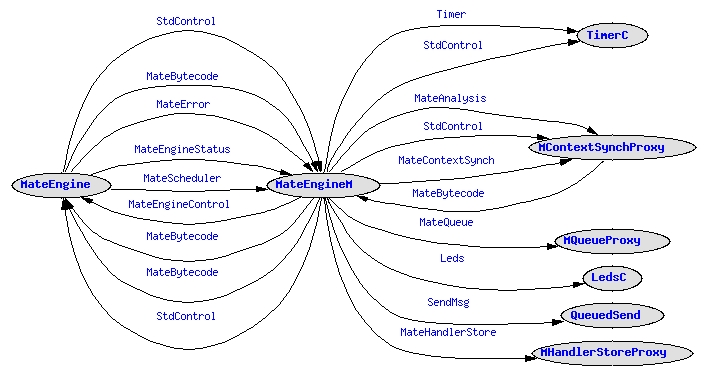
\includegraphics[width=6in]{fig/MateEngine.jpg}
\caption{{\tt MateEngine} wiring diagram.}
\label{fig:mate-engine}
\end{figure}

{\scriptsize
\begin{verbatim}
configuration MateEngine {
  provides {
    interface StdControl;    
    interface MateError as Error;
    interface MateEngineStatus as EngineStatus;
    interface MateScheduler as Scheduler;
    interface MateBytecode as Functions[uint8_t functionID];
  }
  uses {
    interface MateEngineControl as EngineControl;
    interface MateBytecode as Bytecode[uint8_t bytecode];
    interface MateBytecode as FunctionImpls[uint8_t fnID];
    interface StdControl as SubControl;
  }
}
\end{verbatim}
}

Figure~\ref{fig:mate-engine} shows how {\tt MateEngine} wires {\tt
MateEngineM}. {\tt TimerC}, {\tt LedsC}, and {\tt QueuedSend} are all
for when an error condition occurs (triggered by {\tt MateError}):
{\tt MateEngine} starts a periodic timer, blinking the LEDs and
broadcasting the source of the error. {\tt MQueueProxy} is for
manipulating the run queue and {\tt MHandlerStoreProxy} is for
fetching opcodes from handlers.

The set of components that are wired to {\tt MateEngine}'s
parameterized {\tt Bytecode} implement a VM's instruction set. The
main execution loop fetches the next bytecode from a handler (through
the HandlerStore), then dispatches on this interface based on the
opcode value. For example, if the bytecode {\tt halt} has value {\tt
0x2a}, then the {\tt OPhalt} component is wired to {\tt
MateEngine.Bytecode[0x2a]}. Generally, functions included in a VM
(such as {\tt send}) exist as bytecodes.

The {\tt Functions} and {\tt FunctionImpls} are a bit more
complex. First order language (such as motlle) need to be able to
refer to functions by values, which can be stored and passed. The
language then needs a way to take this value and execute the function
it refers to. If a VM supports a first-class language, then all of the
functions must be wired to {\tt FunctionImpls}: the parameters for
this interface are distinct from those for the {\tt Bytecode}
interface. {\tt Functions} is a simple pass-through to {\tt
FunctionImpls}. An instruction component can wire to {\tt
FunctionImpls} to dispatch to a function based on a value.

Any stand-alone component that has to provide {\tt StdControl} should
wire it to {\tt MateEngine}'s {\tt SubControl}. This will allow the VM
to support power management in the future.

{\tt MateEngineM} follows a round-robin FIFO policy. {\tt MateEngineM}
has two configuration constants for timeslicing, {\tt
MATE\_CPU\_QUANTUM} and {\tt MATE\_CPU\_SLICE}. {\tt MateEngineM}
executes instructions in a task. {\tt QUANTUM} is the maximum number
of instructions it interprets in each task execution; {\tt SLICE} is
the number of quanta it gives to a context before switching to a new
one. By default, {\tt MATE\_CPU\_SLICE} is 5 and {\tt
MATE\_CPU\_QUANTUM} is 4. Unless a context halts or blocks, {\tt
MateEngine} timeslices them at the granularity of 20 instructions.

\subsection{Data Model: {\tt MStacks} and {\tt MTypeManager}}

\mate VMs follow a stack architecture. Each thread (execution context)
has an operand stack.  For example, to perform arithmetic addition, a
program pushes two numbers onto the stack, then executes the add
instruction. The add instruction pops the two elements off the stack,
adds them and pushes the result onto the stack. The {\tt MStacks}
component presents the operand stack as an abstract data type.

Operands (and more generally, variables) have an associated type. Some
types, such as integers, are simple. Variables can be more complex
types, such as vectors, lists, or strings. When \mate motes
communicate, they need to take the in-memory representation of a type
and transform it into something that can be sent over a network. For
example, a linked list needs to be compacted into a linear sequence
(i.e., array); the receiver can then unpack the serialized form into
its desired in-memory representation.

{\tt MTypeManager} provides interfaces to the set of
network-compatible types. Specifically, it provides a parameterized
interface (the parameter is the type ID) of type {\tt MateType} (which
is distinct from {\tt MateTypes}, which is type-checking). To
transform a variable between in-memory and network represntations,
components can invoke {\tt MTypeManager}. {\tt MTypeManager}'s
interface is a pass-through to the implementing components: a
component that supports a given type (such as {\tt MBuffer}, which
supports TinyScript's data buffers) wires to {\tt MTypeManager} so
calls will be forwarded properly. If a VM tries to transform a type
for which there is no support, then {\tt MTypeManager} indicates that
the type is not supported: this will generally trigger an error
condition in the VM.

\subsection{Concurrency Management: {\tt MContextSynchProxy}}


\begin{figure}
\centering
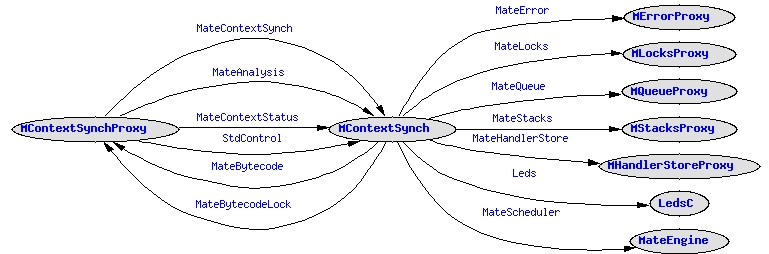
\includegraphics[width=6in]{fig/MContextSynchProxy.jpg}
\caption{{\tt MContextSynchProxy} wiring diagram.}
\label{fig:mcontext-synch-proxy}
\end{figure}

{\tt MContextSynchProxy} is encapsulates {\tt MContextSynch} and wires
it to needed services. {\tt MContextSynch} is responsible for
analyzing code to determine when handlers can safely run
concurrently. ome instructions represent shared resources. For
example, {\tt bpush3} and {\tt getvar4} access shared variables. For
race free program, the VM execution engine must be aware of this and
control scheduling appropriately.

When a component wants a context to run, it submits the
context to {\tt MContextSynch}; based on its analyses, {\tt
MContextSynch} either forwards the context on to {\tt MateEngine} for
execution, or puts it on a wait queue. If a context holding shared
resources halts, {\tt MContextSynch} has it release the resources and
checks if that allows any waiting contexts to run.

{\tt MContextSynch} keeps track of shared resources through the
MateBytecodeLock interface. If an instruction manages a shared
resource, then it must provide this interface. Additionally, in its
ODF, it must have the optional element ``locks'' set to true.

For example, let's look at OPbpush3. This instruction pushes the eight
shared buffers, buffer0-7, onto the operand stack. It is not a library
function; instead, it is an element of the instruction set that
TinyScript compiles to. In {\tt tscript.ldf}
(Section~\ref{sec:language} describes language files in greater
depth), it lists

{\scriptsize
\begin{verbatim}
<OPCODE opcode="bpush3" locks=true>
\end{verbatim}
}

Then, in OPbpush3M:

{\scriptsize
\begin{verbatim}
module OPbpush3M {
  provides interface MateBytecode;
  provides interface MateBytecodeLock;
}
\end{verbatim}
}

{\tt MateBytecodeLock} has a single command:

{\scriptsize
\begin{verbatim}
interface MateBytecodeLock {
  command int16_t lockNum(uint8_t instr);
}
\end{verbatim}
}

This takes a instruction opcode and returns a unique lock
number. The idea is that certain opcodes have a lock associated with
them. {\tt bpush3}, for example, has three bits of embedded operand, for
the eight buffers. If {\tt bpush3 0} is passed to {\tt OPbpush3M.nc},
then it returns the lock number for buffer zero, while {\tt bpush3 1}
will return the lock number for buffer one.

The full {\tt OPbpush1M.nc} logic:

{\scriptsize
\begin{verbatim}
module OPbpush3M {
  ...
  provides interface MateBytecodeLock;
  ...
}


implementation {
  typedef enum {
    BOMB_BUF_LOCK_3_0 = unique("MateLock"),
    BOMB_BUF_LOCK_3_1 = unique("MateLock"),
    ...
    BOMB_BUF_LOCK_3_7 = unique("MateLock"),
  } BufLockNames;
  ...
  command int16_t MateBytecodeLock.lockNum(uint8_t instr) {
    uint8_t which = instr - OPbpush3;
    switch (which) {
    case 0:
      return BOMB_BUF_LOCK_3_0;
    case 1:
      return BOMB_BUF_LOCK_3_1;
    ...
    case 7:
      return BOMB_BUF_LOCK_3_7;
    default:
      return 255;
    }
  }
  ...
}
\end{verbatim}
}

It declares eight unique lock numbers with the nesC unique function. When
lockNum() is called, it returns the lock number associated with the
corresponding buffer. Every context has

{\scriptsize
\begin{verbatim}
  uint8_t heldSet[(BOMB_LOCK_COUNT + 7) / 8];
  uint8_t releaseSet[(BOMB_LOCK_COUNT + 7) / 8];
  uint8_t acquireSet[(BOMB_LOCK_COUNT + 7) / 8];
\end{verbatim}
}

where BOMB\_LOCK\_COUNT is defined to be uniqueCount("MateLock");

\subsubsection{Synchronization Algorithms}

\mate's concurrency manager is responsible for ensuring that handlers
execute atomically. Although it may allow them to run concurrently,
atomicity requires that doing so should be indistinguishable from
their running serially. The concurrency manager maintains a bitmask of
the shared resoures each handler uses (the {\it uses set}), and each
context has three bitmasks: the set of resources it holds (the {\it
held set}), the set of resources it can release (the {\it release
set}), and the set of resources it needs to acquire (the {\it acquire
set}). Initializing a context through {\tt
MateContextSynch.initializeContext} sets a context's acquire set to
its handler's uses set. Every time MContextSynch acquires a lock for a
context, it adds that resource to the context's held set.

When new code for a handler arrives, the concurrency manager runs a
context and flow insensitive program analysis to determine the set of
shared resources that handler uses. It iterates over each instruction
in the handler, using the {\tt MateBytecodeLock} interface to
determine whether an instruction requires a shared resource, updating
the uses set of the handler. 

The concurrency manager maintains a lock for each shared resource;
only one context may access a shared resource. When a component
submits a context to run through the {\tt
MateContextSynch.resumeContext} command, MContextSynch checks the
acquire set of the context. If every resource in the acquire set is
available, MContextSynch atomically acquires all of the locks for the
context and submits it to the scheduler to run. If one or more of the
resources in the context's acquire set are already held, then
MContextSynch puts the context on a wait queue and sets its state to
{\tt MATE\_STATE\_WAITING}.

While they execute, contexts may add resources to their release
set. This does not release those resources. When a context yields,
through the {\tt MateContextSynch.yield} command, MContextSynch has it
unlock each of the resources in its release set, then clears the
set. MContextSynch then tests each context on the wait queue to see if
it is now runnable (the release of locks means all locks in its
acquire set are free). If a context is runnable, MContextSynch resumes
it.

When a context adds a resource to its release set, it may also add it
to its acquire set. This means that the context will release those
resources at the next yield point, but will not continue execution
until it can reacquire them: it can temporarily release the resources.

Currently, TinyScript does not manipulate context release sets,
although it has instructions for doing so. This is an area for future
work.

Because, once it starts running, the acquire set of a context is
always a subset of its release set, the set of resources a context
holds while running is montonically decreasing. A context can never
hold a resource that it did not hold when it started running. This
ensures that contexts can run deadlock-free, while the program
analysis (barring incorrect lock releases at runtime) ensures
race-free execution.


\subsection{Code Propagation: {\tt MHandlerStoreProxy}}


\begin{figure}
\centering
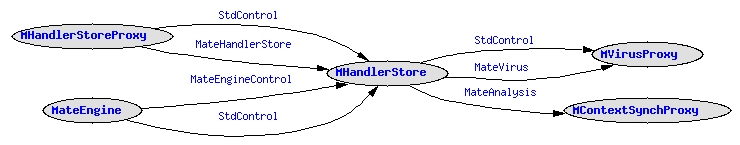
\includegraphics[width=6in]{fig/MHandlerStoreProxy.jpg}
\caption{{\tt MHanderStoreProxy} wiring diagram.}
\label{fig:handler-store}
\end{figure}

The MHandlerStoreProxy component encapsulates \mate's code storage and
propagation. Figure~\ref{fig:handler-store} contains its wiring
diagram, and the component has the following signature:

{\scriptsize
\begin{verbatim}
configuration MHandlerStoreProxy {
  provides {
    interface StdControl;
    interface MateHandlerStore as HandlerStore[uint8_t id];
  }
}
\end{verbatim}
}

Every component that has a handler should wire to HandlerStore, with a
unique ID (the handler ID). VMBuilder automatically generates handler
IDs for contexts, with {\tt unique("MateHandlerID")}; if other
components need to register handlers, they should use the same key for
{\tt unique}.

{\tt MateHandlerStore} has the following signature:

{\scriptsize
\begin{verbatim}
interface MateHandlerStore {
  command result_t initializeHandler();
  command MateHandlerOptions getOptions();
  command MateHandlerLength getCodeLength();
  command MateOpcode getOpcode(uint16_t which);
  event void handlerChanged();
}
\end{verbatim}
}

It provides accessor functions for handlers, and notifies its user
when the code for the handler has changed. Currently, MHandlerStore
allocates a static amount of memory for each handler's code (the
default is 128 bytes), but by controlling access through an interface,
this can easily be changed.

MHandlerStore provides access to code at handler granularity, but
\mate propagates code in terms of capsules, which contain one or more
handlers. The default implementation has a one-to-one handler-capsule
mapping, but languages or compilers may require other
implementations. For example, motlle, due to its semantics, requires
that all handlers propagate together in a single capsule.

MHandlerStore is responsible for triggering program analysis via
MContextSynchProxy when a capsule arrives. MHandlerStore sits on top
of MVirus, which handles capsule propagation. The idea is that a
particular MHandlerStore implementation determines the format of the
data regions of capsules and can parse them into handlers.

\begin{figure}
\centering
\vspace*{-.5cm}
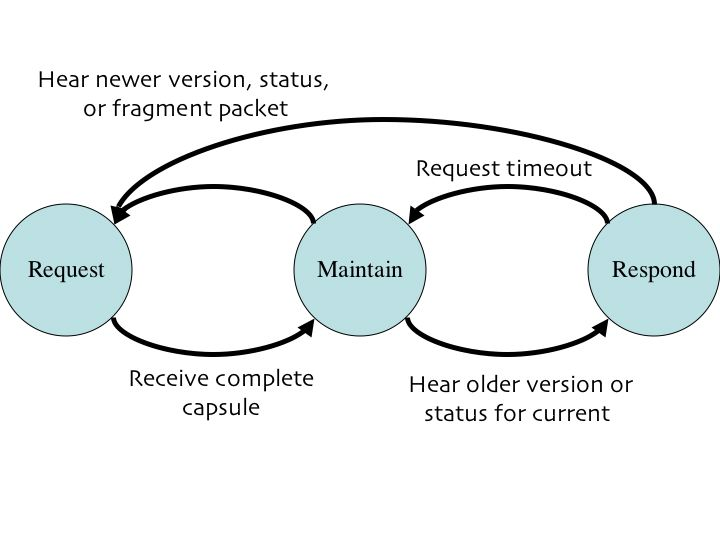
\includegraphics[width=2in]{fig/virus-states.jpg}
\vspace*{-.5cm}
\caption{State diagram for \mate capsule propagation.}
\label{fig:prog_state}
\end{figure}

MVirus uses an epidemic-like approach to propagate capsules: a node
that has newer code will broadcast it to local neighbors. The Trickle
algorithm is used to broadcast three types of data: version packets,
which contain the 32-bit version numbers of all installed capsules,
capsule status packets which describes fragments of a capsule that a
mote needs (essentially, a bitmask), and capsule fragments that are
short segments of a capsule. Figure~\ref{fig:prog_state} contains the
state diagram used by motes for code propagation. A mote can be in one
of three states: maintain (exchanging version packets), request
(sending capsule status packets), or respond (sending
fragments). Nodes start in the maintain state. They enter the request
state if they hear something that indicates someone has a newer
capsule, whether it be a version, capsule status, or fragment
packet. A requesting node returns to the maintain state once it
receives the entire capsule. A node enters the respond state if it is
in the maintain state and hears that someone has an older capsule
(through a version packet), or needs part of its current capsule
(through a capsule status packet). These state transitions mean that
nodes prefer requesting over responding; a node will defer forwarding
capsules until it thinks it is completely up to date.

Trickle's suppression operates on each type of packet (version,
capsule status, and capsule fragment) individually. That is, a capsule
fragment transmission will suppress all other fragment transmissions,
but will not suppress version packets. This allows meta-data exchanges
during propagation: sending a fragment will not cause someone to
suppress a message saying what fragments it needs. Trickling fragments
means that code propagates in a slow and controlled fashion, instead
of as quickly as possible. This is unlikely to significantly disrupt
any existing traffic, and prevents network overload.

\subsubsection{Trickle: The Code Propagation Algorithm}

The Trickle algoithm uses broadcast-based suppressions to quickly
propagate new data but minimize transmissions when nodes share
data. The algorithm operates on an time interval $t$, which has an
upper length of $t_{h}$ and a lower length of $t_{l}$.When an interval
completes, Trickle doubles the size of an interval, up to
$t_{h}$. When it learns of new code (e.g., by overhearing a capsule
fragment, version vector, or capsule status packet with a higher
version number), it shrinks the interval to $t_{l}$.

Essentially, when there's nothing new to say, \mate VMs gossip
infrequently: $\tau$ is set to $\tau_{h}$. However, as soon as a mote
hears something new, it gossips more frequently, so those who haven't
heard it yet find out. The chatter then dies down, as $\tau$ grows
from $\tau_{l}$ to $\tau_{h}$.

Trickle maintains a redundancy constant $k$ and a counter
$c$. Whenever it hears a packet that would suppress its own
transmission (e.g., a capsule fragment if in the respond state), it
increments $c$. At the beginning of an interval, the algorithm resets
$c$ to zero, and picks a random time in the range of
$[\frac{t}{2},t]$. When it reaches that time, it transmits data if and
only if $c < k$. 

\section{\mate Operations}

MateEngine executes programs in terms of operations. Every operation
has one or more one-byte opcodes, which map to a component that
implements the {\tt MateBytecode} interface. An operation can have
embedded operands, which cause it to exist as more than one
opcode. For example, the {\tt bpush3} operation (which the TinyScript
language uses) has three bits of embedded operand, corresponding to
the eight data buffers TinyScript makes available.

The \mate tutorials describe how to write new functions, which are a
particular kind of operation: they never have embedded operands, and
are generally expected to provide language-independent
functionality. In addition to functions, operations can also be
primitives, which are the operations that compose a language. This is
why function components have the prefix ``OP,'' such as {\tt OPid}.


\subsection{Operation Component Naming Convention}

Operation components have the following naming convention:

{\scriptsize
\begin{verbatim}
    OP<width><name><operand>.nc
\end{verbatim}
}

Width and operand are both numbers. Width specifies how many bytes
wide the instruction is. If no width is specified, the default is
one. Operand specifies how many bytes of embedded operand there
are. If no operand is specified, the default is zero. Note that, after
considering width and operand, the instruction must have an opcode in
its first byte. That is, the instruction cannot be two bytes wide and
have no embedded operand; as the \mate scheduler dispatches on the
first byte of the opcode, it would not be able to distinguish this
instruction from other ones.

Here are a few examples:

\vspace{0.1in}
{\scriptsize
\begin{tabular}{|l|c|c|c|l|} \hline
Component & Width & Name  & Embedded & Description\\ \hline
OPrand    &  1    & rand  & 0        & Generates a random number\\
OPpushc6  &  1    & pushc & 6        & Push a constant onto the stack\\
OP2jumps10&  2    & jumps & 10       & Jump to a 10-bit address\\ \hline
\end{tabular}
}
\vspace{0.1in}

Functions are always one byte wide and never have embedded
operands. In the above example, neither {\tt pushc} nor {\tt jumps}
are available as library functions; they are actually primitives that
compose part of what TinyScript compiles to.

\subsection{Primitives}

Primitives are operation components that a language compiles to. They
cannot be included in a VM in the same way functions can: they have no
ODF which VMBuilder can use to include them. The only way to include
them is to use a language that compiles to them. Operations such as
branches, memory access, and arithmetic are examples of \mate
primitives.

Primitives provide language storage abstractions, such as
variables. For example, TinyScript has the notion of sixteen variables
that are shared between all handlers, and eight variables which are
private to each handler. The operations {\tt getvar4} and {\tt
setvar4} implement the former, while the operations {\tt getlocal3}
and {\tt setlocal3} implement the latter.

The implementations of the two abstractions are very similar. A single
component implements {\tt getvar4} and {\tt setvar4}, providing two
{\tt MateBytecode} interfaces. Sixteen opcodes map to each instance of
{\tt MateBytecode}, for the four bits of embedded operand. The
component allocates sixteen shared variables in its frame.  To
determine which variable a program is accessing, the implementation
subtracts the executed opcode from the base opcode, Additionally, the
implementation checks that the program holds the lock to the shared
variable:

{\scriptsize
\begin{verbatim}
  MateStackVariable heap[16];

  command result_t Get.execute(uint8_t instr,
                               MateContext* context) {
    uint8_t arg = instr - OPgetvar4;
    uint8_t lock = varToLock(arg);
    if ((lock == 255) || !call Locks.isHeldBy(lock, context)) {
      call Error.error(context, MATE_ERROR_INVALID_ACCESS);
      return FAIL;
    }
    dbg(DBG_USR1, "VM (%i): Executing getvar (%i).\n", (int)context->which, (int
)arg);
    call Stacks.pushOperand(context, &heap[arg]);
    return SUCCESS;
  }
\end{verbatim}
}

{\tt getlocal3} and {\tt setlocal3} are similar, except there
are only eight variables, and there's no need to check locks. However,
the component that implements the two primitives has to allocate state
for each context:

{\scriptsize
\begin{verbatim}
  MateStackVariable vars[MATE_CONTEXT_NUM][NUM_VARS];

  command result_t Get.execute(uint8_t instr,
                               MateContext* context) {
    uint8_t arg = instr - OPgetlocal3;
    dbg(DBG_USR1, "VM (%i): OPgetlocal3 (%i).\n", (int)context->which, (int)arg)
;
    call Stacks.pushOperand(context, &vars[context->which][arg]);
    return SUCCESS;
  }
\end{verbatim}
}

Some primitives are more than one byte wide. For example, {\tt
OP2jumps10}, the basic branch instruction is two bytes wide. The {\tt
byteLength()} command of the {\tt MateBytecode} interface must return
the byte width of an instruction, so the scheduler knows how much to
increment the program counter by. {\tt It increments the program
counter before executing the instruction.} The component implementing
the primitive is responsible for getting the extra bytes. For example,
this is part of {\tt OP2jumps10M}:

{\scriptsize
\begin{verbatim}
  command uint8_t MateBytecode.byteLength() {return 2;}

  command result_t MateBytecode.execute(uint8_t instr,
                                            MateContext* context) {
    uint16_t addr = (instr - OP2jumps10) << 8;
    MateStackVariable* cond = call Stacks.popOperand(context);

    addr |= call Store.getOpcode[context->currentHandler](context->pc-1);
\end{verbatim}
}

It generates the 10-bit jump address by taking the bottom two bits of
the opcode and incorporating the next byte. Since the VM has already
incremented the program counter, the next byte is at {\tt context-$>$pc-1}.

The \mate tutorials briefly mention a requirement when using the \mate
operand stack. When a component pops operands off the stack with {\tt
popOperand}, the call returns a pointer to a stack variable. This is a
pointer into the stack data structure. If a component then pushes
something onto the stack, that push can modify the region of the stack
the pointer refers to. There are situations when it is safe to access
popped operands after pushes, however.

Elements on the operand stack have a fixed size. For example, a buffer
(which stores a pointer) is the same size as a value. An operand stack
is an array of operands and a stack pointer, which indicates the next
free element. Pushing something onto the stack fills the next free
element, and increments the stack pointer. Popping something off the
stack decrements the stack pointer, and returns a pointer to that
element. The following three snippets of pseudocode are examples of
the resulting behavior:

\begin{verbatim}
  op1 = pop();
  op2 = pop();
  push(4);   // op2 is now invalidated
  push(op2); // BUG, unless you want to copy the top of the operand stack

  op1 = pop();
  op2 = pop();
  push(op2);  // SAFE; returns op2 to operand stack
  push(op1);  // same as above

  op1 = pop();
  op2 = pop();
  push(op1); // invalidates op2, which is now the same as op1
  push(4);   // invalidates op1
\end{verbatim}


\section{Languages}
\label{sec:language}

A language is defined by the set of primitives it compiles to. A
LANGUAGE element in a VM specification file causes VMBuilder to search
for a language description file ({\tt .ldf}). An LDF must have a
LANGUAGE element with the NAME and DESC tags. Additionally, it should
have a series of PRIMITIVE elements.  PRIMITIVE elements have one
required tag, OPCODE. They also have the optional field LOCKS, which
specifies if the primitive encapsulates a shared resources which the
concurrency manager must arbitrate access to. For example, this is a
snippet of {\tt tscript.ldf}:

{\scriptsize
\begin{verbatim}
<LANGUAGE name="TinyScript" desc="A simple, BASIC-like language.">
<PRIMITIVE opcode="halt">
<PRIMITIVE opcode="2pushc10">
<PRIMITIVE opcode="2jumps10">
<PRIMITIVE opcode="getlocal3">
<PRIMITIVE opcode="setlocal3">
<PRIMITIVE opcode="bpush3" locks=true>
<PRIMITIVE opcode="getvar4" locks=true>
<PRIMITIVE opcode="setvar4" locks=true>
<PRIMITIVE opcode="or">
<PRIMITIVE opcode="and">
<PRIMITIVE opcode="not">
<PRIMITIVE opcode="eq">
<PRIMITIVE opcode="gte">
<PRIMITIVE opcode="gt">
\end{verbatim}
}

VMBuilder interprets PRIMITIVE elements in a language file; it does
not load any additional files in response to them. It uses the OPCODE
tag to refer to the primitive's component when wiring the instruction
set. If the LOCKS tag exists (the value is ignored), the VMBuilder
also has MateTopLevel wire the primitive component to the concurrency
manager.

The LANGUAGE element has a single optional tag,
FIRSTORDERFUNCTIONS. If the LANGAUGE element has this tag (whose value
is ignored), the VMBuilder includes support for first order
functions. It does so by wiring functions to the {\tt FunctionImpls}
interface of {\tt MateEngine} and generating a set of function
identifiers of the form fn\_name, where {\it name} is the name of the
function. These indentifiers are in an enum in {\tt MateConstants.h},
and can therefore can be accessed through the VM Java constants file.

\section{VM Options}

Tutorial 4 presents how to specify the language, events, and functions
that a \mate VM supports. More advanced users can also modify various
VM options. These options can be set with one or more {\tt OPTION}
elements. The supported options are:

\vspace{1ex}
{\scriptsize
\begin{tabular}{|l|l|l|}\hline
Name  & Type & Description \\ \hline
OPDEPTH      & integer & Sets the maximum depth of a context operand stack. \\
             &         & The default value is 8.\\
             &         & Changing this value will change the maximum length of  TinyScript statements.\\
             &         & Larger values increase RAM utilization.\\\hline
BUF\_LEN      & integer & Sets the maximum size of a data buffer.\\
             &         & The default value is 10.\\
	     &         & Larger values will allow you to manage larger buffers. \\
             &         & However, this will increase the RAM allocated for each buffer.\\
             &         & If made much larger, it increase packet size, {\bf greatly} increasing RAM utilization.\\
             &         & Decreasing this value will not reduce the RAM utilization of message buffers.\\ \hline
CAPSULE\_SIZE & integer & Sets the maximum size of a code capsule.\\
             &         & The default value is 128.\\
             &         & Changing this value will affect how large a program you can write.\\
             &         & Larger values increase RAM utilization.\\ \hline
DELUGE       & string  & Support Deluge binary reprogramming. \\ \hline
             &         & The string specified is ignored. \\
             &         & Including this option will incorporate Deluge binary reprogramming. \\
             &         & Full information on Deluge can be found in the Deluge manual, \\
             &         & which is part of the a standard TinyOS release.\\
             &         & Deluge uses roughly 10kB of code memory and 250B of RAM. \\\hline
\end{tabular}
}
\vspace{1ex}

For example, to change some options, you could add either a single element

\begin{verbatim}
<OPTION OPDEPTH=6 CAPSULE_SIZE=64>
\end{verbatim}

or multiple elements

\begin{verbatim}
<OPTION OPDEPTH=6>
<OPTION CAPSULE_SIZE=64>
\end{verbatim}



\section{Java Toolchain}

When VMBuilder generates a Makefile for a \mate VM, it includes rules
for building a few Java classes that the \mate toolchain uses. The
foremost of these is a constants class, which it generates with the
{\tt ncg} tool. This class contains all of the mappings between
handler names and IDs, context names and IDs, instructions and their
bytecodes, error codes, and data types. It also generates a set of
message classes, for interacting with a VM.

\subsection{Constants Class}

Every VM has a constants class. The name of the class is VM-specific,
to prevent users from accidentally loading the wrong constants
file. For example, the Bombilla constants class name is
BombillaConstants. The class contains all of the constants contained
in MateConstants.h as public variables. The \mate toolchain has a
class, named {\tt net.tinyos.script.ConstantMapper}, for easily
accessing these variables through the Java reflection API.

The constructor to ConstantMapper takes two arguments, a class name
and a prefix. The prefix acts as a filter on the constants it
considers. For example, if you instantiate a ConstantMapper like so:

\begin{verbatim}
ConstantMapper map = new ConstantMapper("BombillaConstants", "OP");
\end{verbatim}

then all of its accessor functions will operate on the public fields
of a class named {\tt BombillaConstants} whose name begins with {\tt
OP}, in this case the instructions of the Bombilla VM.

ConstantMapper provides three basic methods for fetching constants:
{\tt codeToName()} {\tt nameToCode()}, and {\tt names()}. For example,
the TinyScript compiler takes a TinyScript program and produces
assembly code for it. The ScriptAssembler then takes each instruction
and determines its bytecode with the {\tt nameToCode()} method. In
contrast, when the Scripter displays a VM error, it reads the binary
values of the error condition, context, and handler, and produces
human-readable names for them with the {\tt codeToName()}
method. Finally, the ScripterGUI determines the set of valid handlers
one can write scripts for by using {\tt names()}, then translates
those names to IDs with {\tt nameToCode()}.

Obtaining the name of a VM's constants file requires reading in the VM
description file that VMBuilder produces. Every VM application
directory has a file named {\tt vm.vmdf}, which describes the VM. The
Java class {\tt net.tinyos.script.Configuration} automatically loads
and parses VM descroption files, extracting the important fields. It
takes the path to the file as an argument in its constructor. This is
why you must run Scripter from the VM application directory: it
instantiates a Configuration with the name {\tt vm.vmdf}. This will
also ensure that the Java loader will find the right constants
file. Configuration has accessor functions to get at the important
instances of ConstantMapper, such as capsule names, opcodes, and error
codes. You can also get the constant class name, if you need to build
other ConstantMappers, with the {\tt constantClassName()} method.


\subsection{Message Classes}

By default, the Makefile VMBuilder generates builds several Java
message classes. These classes are all built in the {\tt vm\_specific}
subdirectory. They allow Scripters to generate the proper packets for
transmitting code to a mote, as well as read mote data output.

The first class, code transmission, has three kinds of messages: {\tt
CapsuleMsg}, {\tt CapsuleStatusMsg}, and {\tt
CapsuleChunkMsg}. CapsuleMsg is for generating a full \mate capsule
that matches the on-mote memory layout. CapsuleStatusMsg is so tools
can monitor download status as it occurs. CapsuleChunkMsg is so the
Scripters can send the chunks that make up a capsule along the serial
port to a mote.

The second class, data transmission, has three kinds of messages: {\tt
BufferBCastMsg}, {\tt BufferUARTMsg}, and {\tt MultiHopMsg}. The first
two are the format the {\tt bcast} and {\tt uart} functions send: a
\mate data buffer in the payload of a packet. MultiHopMsg is for
packets sent through a multihop routing layer: it includes multihop
header fields, as well as the \mate buffer. The tool {\tt
net.tinyos.script.VMBufferReader} listens for all three of these kinds
of packets and outputs information on them. It is a good place to
start if you want to read data from \mate into a Java application.


\section{Conclusion}

\mate is under active development. Bugs, questions, contexts, and
functions can be sent to Phil Levis ({\tt pal@cs.berkeley.edu}).

\end{document}
